% !TeX root = ./../main.tex

\section{Rysunki uzupełniające do rozdziału~\ref{chapter:pdu}}\label{app:results:pdu2}
\agentinfo{
Sekcja utworzona w zadaniu PHD-TS-97 (2026-11-27, skracanie rozdziału 4 z 18 do 16 stron); wykaz cięć: \agentref{eksperymenty/recenzje/rozdzial-4-skracanie.md}.
Zawiera dwa rysunki przeniesione z rozdziału 4 bez zmian treści i podpisów (trzeci, schemat blokowy fig:pdu:flowchart, wrócił do sekcji 4.5 decyzją autora z 2026-11-28): fig:pdu:pearson (z sekcji 4.7.3) i fig:pdu:two-comp (z sekcji 4.7.4).
Pierwszy powtarza w postaci graficznej treść, która w rozdziale pozostała (wartości r z tabel tab:pdu:corr i tab:pdu:app:iccs); drugi jest przykładem do eksperymentu E4, którego wynik rozdział opisuje jako jakościowy.
Wiersz input dla tego pliku dopisuje orkiestrator w pliku chapters/appendix_results.tex (po sekcji app:results:pdu).
}
\agenttask{
Pytanie do autora (skracanie rozdziału 4, zadanie PHD-TS-97): czy wykres fig:pdu:pearson i przykład fig:pdu:two-comp mają zostać w dodatku, czy któryś z nich ma wrócić do rozdziału 4? Schemat blokowy fig:pdu:flowchart wrócił do sekcji 4.5 decyzją autora z 2026-11-28.
Powrót kosztuje około 0,4 strony (wykres) albo 0,3 strony (przykład); po przywróceniu schematu rozdział ma 16 stron i 6 wierszy na siedemnastej, co autor zaakceptował 2026-11-28 (plik eksperymenty/recenzje/rozdzial-4-skracanie.md).
}

Sekcja zawiera dwa rysunki do rozdziału~\ref{chapter:pdu}.
Rysunek~\ref{fig:pdu:pearson} przedstawia współczynniki korelacji Pearsona z tabel~\ref{tab:pdu:corr} i~\ref{tab:pdu:app:iccs}, omawiane w podrozdziałach~\ref{subsec:pdu:results:one} i~\ref{subsec:pdu:results:two}, a rysunek~\ref{fig:pdu:two-comp} przykład korekty szeregu dwuskładnikowego w eksperymencie E4 (podrozdział~\ref{subsec:pdu:results:two}).


\begin{figure}[htbp]
\centering
% !TeX root = ./../../main.tex
% Współczynnik korelacji Pearsona przed korektą i po korekcie funkcją PDU (rysunek fig:pdu:pearson).
% Wykres odtworzony w pgfplots z danych liczbowych; żadna wartość nie została odczytana z wykresu źródłowego.
% Dane (a), funkcje jednej zmiennej:
%   zbiór z pracy magisterskiej: artykuły/magisterka_werner_final/chapters/03.tex, tabela tab:pearson_coefficients
%     oraz zdanie pod tabelą (łącznie 10 086 próbek: 0.761 -> 0.987);
%   zbiór z artykułu ICCS 2022: artykuły/Quantum_Errors_ICCS/imgs/pearson.png (wiersze ,,original results'' i ,,correction level'';
%     wartość po korekcie = suma obu wierszy); plik pearson.png leży w katalogu artykułu, ale nie jest włączony w main.tex;
%     wartości 0.876, 0.9707 i przyrosty dla Athens, Quito, Lima, Manila są też w tekście artykułu (sekcja Results).
% Dane (b), funkcja dwóch zmiennych: artykuły/magisterka_werner_final/chapters/03.tex, tabela tab:pearson_coefficients_seven
%   oraz zdanie nad tabelą (łącznie 21 760 próbek: 0.507 -> 0.418).
% Wymaga: pgfplots z biblioteką groupplots (wczytane w config/my-settings.tex).
\begin{tikzpicture}
\begin{groupplot}[
  group style={group size=2 by 1, horizontal sep=1.6cm},
  height=4.6cm,
  ymajorgrids,
  grid style={black!15},
  tick label style={font=\footnotesize},
  label style={font=\footnotesize},
  title style={font=\footnotesize, yshift=-1mm},
  xticklabel style={rotate=40, anchor=east, font=\footnotesize},
  yticklabel style={/pgf/number format/.cd, fixed, fixed zerofill, precision=1, use comma},
  ylabel={współczynnik Pearsona $r$},
]
% ---------- (a) funkcje jednej zmiennej ----------
\nextgroupplot[
  width=0.60\textwidth,
  title={(a) funkcje jednej zmiennej},
  xmin=0.4, xmax=8.6,
  ymin=0.6, ymax=1.02,
  xtick={1,...,8},
  xticklabels={Athens,Belem,Bogota,Lima,Manila,Quito,Santiago,łącznie},
  ytick={0.6,0.7,0.8,0.9,1.0},
  legend to name=pdupearsonlegend,
  legend style={font=\footnotesize, legend columns=2, draw=none, /tikz/every even column/.append style={column sep=4mm}},
]
% odcinki łączące wartość przed korektą i po korekcie: praca magisterska
\addplot[black, forget plot] coordinates {(0.82,0.978) (0.82,0.981)};
\addplot[black, forget plot] coordinates {(1.82,0.836) (1.82,0.966)};
\addplot[black, forget plot] coordinates {(2.82,0.646) (2.82,0.978)};
\addplot[black, forget plot] coordinates {(3.82,0.892) (3.82,0.997)};
\addplot[black, forget plot] coordinates {(4.82,0.855) (4.82,0.976)};
\addplot[black, forget plot] coordinates {(5.82,0.913) (5.82,0.994)};
\addplot[black, forget plot] coordinates {(6.82,0.875) (6.82,0.990)};
\addplot[black, forget plot] coordinates {(7.82,0.761) (7.82,0.987)};
% odcinki: artykuł ICCS 2022
\addplot[black!55, forget plot] coordinates {(1.18,0.9787) (1.18,0.9819)};
\addplot[black!55, forget plot] coordinates {(2.18,0.8364) (2.18,0.9661)};
\addplot[black!55, forget plot] coordinates {(3.18,0.8866) (3.18,0.9712)};
\addplot[black!55, forget plot] coordinates {(4.18,0.8983) (4.18,0.9711)};
\addplot[black!55, forget plot] coordinates {(5.18,0.8203) (5.18,0.9641)};
\addplot[black!55, forget plot] coordinates {(6.18,0.9538) (6.18,0.9836)};
\addplot[black!55, forget plot] coordinates {(7.18,0.9785) (7.18,0.9884)};
\addplot[black!55, forget plot] coordinates {(8.18,0.8760) (8.18,0.9707)};
% praca magisterska: przed korektą i po korekcie
\addplot[only marks, mark=o, mark size=2.2pt, black, fill=white] coordinates {(0.82,0.978) (1.82,0.836) (2.82,0.646) (3.82,0.892) (4.82,0.855) (5.82,0.913) (6.82,0.875) (7.82,0.761)};
\addlegendentry{praca magisterska, przed korektą}
\addplot[only marks, mark=*, mark size=2.2pt, black] coordinates {(0.82,0.981) (1.82,0.966) (2.82,0.978) (3.82,0.997) (4.82,0.976) (5.82,0.994) (6.82,0.990) (7.82,0.987)};
\addlegendentry{praca magisterska, po korekcie}
% artykuł ICCS 2022: przed korektą i po korekcie
\addplot[only marks, mark=square, mark size=2pt, black!55] coordinates {(1.18,0.9787) (2.18,0.8364) (3.18,0.8866) (4.18,0.8983) (5.18,0.8203) (6.18,0.9538) (7.18,0.9785) (8.18,0.8760)};
\addlegendentry{artykuł ICCS 2022, przed korektą}
\addplot[only marks, mark=square*, mark size=2pt, black!55] coordinates {(1.18,0.9819) (2.18,0.9661) (3.18,0.9712) (4.18,0.9711) (5.18,0.9641) (6.18,0.9836) (7.18,0.9884) (8.18,0.9707)};
\addlegendentry{artykuł ICCS 2022, po korekcie}
% ---------- (b) funkcja dwóch zmiennych ----------
\nextgroupplot[
  width=0.38\textwidth,
  title={(b) funkcja dwóch zmiennych},
  xmin=0.4, xmax=5.6,
  ymin=0.3, ymax=0.72,
  xtick={1,...,5},
  xticklabels={Lagos,Casablanca,Perth,Jakarta,łącznie},
  ytick={0.3,0.4,0.5,0.6,0.7},
  ylabel={},
]
\addplot[black, forget plot] coordinates {(1,0.378) (1,0.355)};
\addplot[black, forget plot] coordinates {(2,0.691) (2,0.522)};
\addplot[black, forget plot] coordinates {(3,0.525) (3,0.491)};
\addplot[black, forget plot] coordinates {(4,0.506) (4,0.363)};
\addplot[black, forget plot] coordinates {(5,0.507) (5,0.418)};
\addplot[only marks, mark=o, mark size=2.2pt, black, fill=white] coordinates {(1,0.378) (2,0.691) (3,0.525) (4,0.506) (5,0.507)};
\addplot[only marks, mark=*, mark size=2.2pt, black] coordinates {(1,0.355) (2,0.522) (3,0.491) (4,0.363) (5,0.418)};
\end{groupplot}
\node[anchor=north] at ($(group c1r1.south)!0.5!(group c2r1.south)+(0,-1.25cm)$) {\pgfplotslegendfromname{pdupearsonlegend}};
\end{tikzpicture}

\caption[Współczynnik korelacji Pearsona przed korektą i po korekcie funkcją PDU]{Współczynnik korelacji Pearsona między wynikami a wartościami oczekiwanymi przed korektą (znaczniki puste) i po korekcie funkcją PDU (znaczniki pełne): (a)~funkcje jednej zmiennej według dwóch zbiorów danych, (b)~funkcja dwóch zmiennych.
Opracowanie własne na podstawie danych z~prac~\cite{werner_experiment_driven_2022,werner_magisterka_2022}.}
\label{fig:pdu:pearson}
\end{figure}

\begin{figure}[htbp]
\centering
\begin{tabular}{@{}ccc@{}}
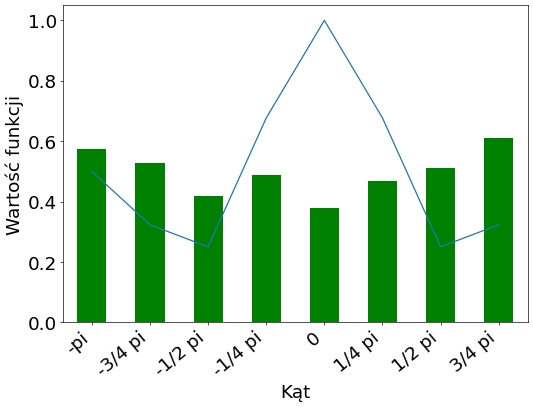
\includegraphics[width=0.29\textwidth]{figures/chp_pdu/pdu_lima_two_comp_before.png} &
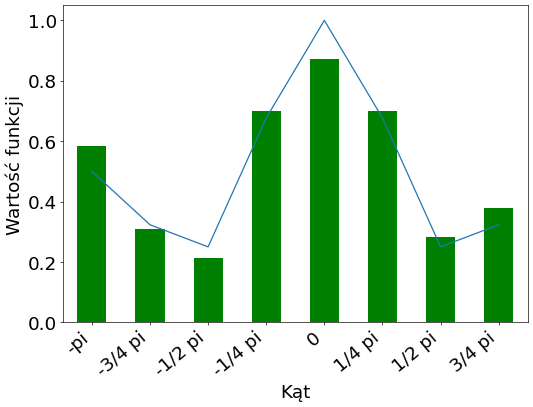
\includegraphics[width=0.29\textwidth]{figures/chp_pdu/pdu_lima_two_comp_after.png} &
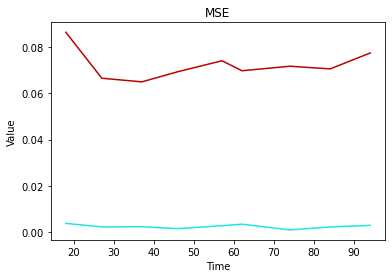
\includegraphics[width=0.29\textwidth]{figures/chp_pdu/pdu_lima_two_comp_mse.png}
\end{tabular}
\caption[Korekta szeregu dwuskładnikowego na urządzeniu Lima]{Szereg dwuskładnikowy $\tfrac{1}{2}(\coscomp_{1,0}+\coscomp_{2,0})$ na urządzeniu Lima: wartości przed korektą (po lewej) i po korekcie (w środku) na tle wartości oczekiwanych (linia) oraz błąd średniokwadratowy kolejnych serii w~funkcji czasu w~minutach (po prawej; linia czerwona przed korektą, turkusowa po korekcie).
Według nazw plików źródłowych słupki pochodzą z~19.06.2022, a~przebieg błędu z~19.01.2022.
Rysunki własne autora, przeniesione z~pracy~\cite{werner_magisterka_2022}.}
\label{fig:pdu:two-comp}
\end{figure}
% ŹRÓDŁO dat w podpisie: nazwy plików w artykuły/magisterka_werner_final/chapters/03.tex, rysunki fig:qCoSamp_multi (result_2_06_19_2022_14_11_13_ibmq_lima_cosphi2phi.png, correctedResult_2_06_19_2022_14_10_45_ibmq_lima_cosphi2phi.png) i fig:qCoSamp_multi_mse (01_19_2022_02_27_24_ibmq_lima_MSE_cos_phi.png).
